
\mode<presentation> {

% The Beamer class comes with a number of default slide themes
% which change the colors and layouts of slides. Below this is a list
% of all the themes, uncomment each in turn to see what they look like.

%\usetheme{default}
%\usetheme{AnnArbor}
%\usetheme{Antibes}
%\usetheme{Bergen}
%\usetheme{Berkeley}
%\usetheme{Berlin}
%\usetheme{Boadilla}
%\usetheme{CambridgeUS}
%\usetheme{Copenhagen}
%\usetheme{Darmstadt}
%\usetheme{Dresden}
%\usetheme{Frankfurt}
%\usetheme{Goettingen}
%\usetheme{Hannover}
%\usetheme{Ilmenau}
%\usetheme{JuanLesPins}
%\usetheme{Luebeck}
%\usetheme{Madrid}
%\usetheme{Malmoe}
%\usetheme{Marburg}
%\usetheme{Montpellier}
\usetheme{PaloAlto}
%\usetheme{Pittsburgh}
%\usetheme{Rochester}
%\usetheme{Singapore}
%\usetheme{Szeged}
%\usetheme{Warsaw}

% As well as themes, the Beamer class has a number of color themes
% for any slide theme. Uncomment each of these in turn to see how it
% changes the colors of your current slide theme.

%\usecolortheme{albatross}
%\usecolortheme{beaver}
%\usecolortheme{beetle}
%\usecolortheme{crane}
%\usecolortheme{dolphin}
%\usecolortheme{dove}
%\usecolortheme{fly}
%\usecolortheme{lily}
%\usecolortheme{orchid}
%\usecolortheme{rose}
%\usecolortheme{seagull}
%\usecolortheme{seahorse}
%\usecolortheme{whale}
%\usecolortheme{wolverine}

%\setbeamertemplate{footline} % To remove the footer line in all slides uncomment this line
%\setbeamertemplate{footline}[page number] % To replace the footer line in all slides with a simple slide count uncomment this line

%\setbeamertemplate{navigation symbols}{} % To remove the navigation symbols from the bottom of all slides uncomment this line
}

% remove title and author from left panel
 \makeatletter
  \setbeamertemplate{sidebar \beamer@sidebarside}%{sidebar theme}
  {
    \beamer@tempdim=\beamer@sidebarwidth%
    \advance\beamer@tempdim by -6pt%
    \insertverticalnavigation{\beamer@sidebarwidth}%
    \vfill
    \ifx\beamer@sidebarside\beamer@lefttext%
    \else%
      \usebeamercolor{normal text}%
      \llap{\usebeamertemplate***{navigation symbols}\hskip0.1cm}%
      \vskip2pt%
    \fi%
  }%
\makeatother
% done remove title and author from left panel 

\hypersetup{colorlinks,citecolor=}
\usepackage{graphicx} % Allows including images
\usepackage{booktabs} % Allows the use of \toprule, \midrule and \bottomrule in tables
\usepackage{natbib}
\usepackage{apalike}
\usepackage{comment}
% \usepackage{enumitem}
% \setlist[itemize]{topsep=0pt,before=\leavevmode\vspace{-1.5em}}
% \setlist[description]{style=nextline}
\usepackage{amsthm}
\usepackage{media9}
% \usepackage{multimedia}
\usepackage{hyperref}
\usepackage{tikz}
\tikzset{
     arrow/.style={-{Stealth[]}}
     }
\usetikzlibrary{positioning,arrows.meta}
\usetikzlibrary{shapes.geometric}

\setbeamertemplate{navigation symbols}{}%remove navigation symbols

\usepackage{setspace}

\newtheorem{probDef}{Definition}
\newtheorem*{probDef*}{Definition}
\newtheorem{claim}{Claim}
\newtheorem*{claim*}{Claim}
\newtheorem{probExample}{Example}
\newtheorem{probRule}{Rule}
\newtheorem{probAxiom}{Axiom}
\setbeamertemplate{theorems}[numbered]

\newtheorem{manualprobRuleinner}{Rule}
\newenvironment{manualProbRule}[1]{%
  \renewcommand\themanualprobRuleinner{#1}%
  \manualprobRuleinner
}{\endmanualprobRuleinner}

\newtheorem{manualprobExampleinner}{Example}
\newenvironment{manualProbExample}[1]{%
  \renewcommand\themanualprobExampleinner{#1}%
  \manualprobExampleinner
}{\endmanualprobExampleinner}

\newcounter{saveenumi}
\newcommand{\seti}{\setcounter{saveenumi}{\value{enumi}}}
\newcommand{\conti}{\setcounter{enumi}{\value{saveenumi}}}
\newcommand{\keepi}{\addtocounter{saveenumi}{-1}\setcounter{enumi}{\value{saveenumi}}}

%----------------------------------------------------------------------------------------
%	TITLE PAGE
%----------------------------------------------------------------------------------------

\title{Foundations of probability theory}

\author{Joaqu\'{i}n Rapela} % Your name
\institute[GCNU, UCL] % Your institution as it will appear on the bottom of every slide, may be shorthand to save space
{
Gatsby Computational Neuroscience Unit\\University College London % Your institution for the title page
}
\date{\today} % Date, can be changed to a custom date

\AtBeginSection[]
  {
     \begin{frame}<beamer>
     \frametitle{Contents}
         \tableofcontents[currentsection,hideallsubsections]
     \end{frame}
  }

\begin{document}

\begin{frame}
\titlepage % Print the title page as the first slide
\end{frame}

\begin{frame}
\frametitle{Contents} % Table of contents slide, comment this block out to remove it
\tableofcontents % Throughout your presentation, if you choose to use \section{} and \subsection{} commands, these will automatically be printed on this slide as an overview of your presentation
\end{frame}

\begin{frame}
\frametitle{Main reference} % Table of contents slide, comment this block out to remove it

    I will mainly follow chapters seven \textit{Foundations of probability
    theory} and eight \textit{Conditional probability and Bayes} from
    \citet{tijms12}.

    \begin{center}
        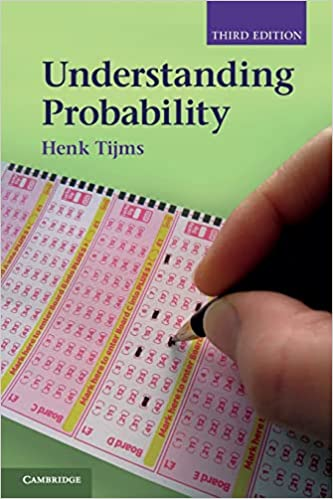
\includegraphics[width=1.5in]{figures/tijms12UnderstandingProbabilityCover.jpg}
    \end{center}

\end{frame}

\begin{frame}
\frametitle{Main lecture goals}

    % \resizebox{5}{3}{%
    % \scalebox{0.7}{%
    \begin{figure}
        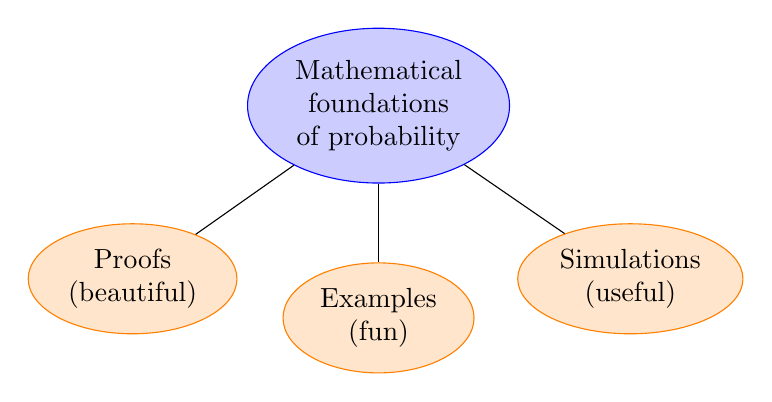
\begin{tikzpicture}
            % Place nodes
            \node[ellipse,align=center,anchor=north,fill=blue!20,draw=blue] (foundations) {Mathematical\\foundations\\of probability};
            \node[ellipse,align=center,anchor=north,fill=orange!20,draw=orange] [below left=of foundations] (proofs) {Proofs\\(beautiful)};
            \node[ellipse,align=center,anchor=north,fill=orange!20,draw=orange] [below=of foundations] (examples) {Examples\\(fun)};
            \node[ellipse,align=center,anchor=north,fill=orange!20,draw=orange] [below right=of foundations] (simulations) {Simulations\\(useful)};
            % Draw edges
            \path[-] (foundations) edge node [] {} (proofs);
            \path[-] (foundations) edge node [] {} (examples);
            \path[-] (foundations) edge node [] {} (simulations);
        \end{tikzpicture}
    \end{figure}
    % }

\end{frame}

\section{Foundations of probability theory}

\subsection{Historical notes}

\begin{frame}
\frametitle{Historical notes}

\small
\begin{description}

    \item[Gerolamo Cardano (1501-1576)] first mathematical analysis of games of chance, introduced probability as the ratio between favorable and the total number of possible outcomes

    \item[Pierre Fermat and Blaise Pascal (1654)] correspondence about the solution of a problem posed by the Chevalier de Mere established the basic principles of probability.

    \item[Christian Huygen (1629-1695)] laid the foundations of current probabity theory. Introduced the concept of expected value.

    \item[Pierre Simon Laplace (1749-1827)] published \textit{Theorie Analytique dez Probabilities}, the greatest contribution in the history of probability.

    \item[Andrej Kolmogorov (1903-1987)] laid the current axiomatic foundation of probability.

\end{description}
\normalsize

\end{frame}

\begin{comment}
- explain the frequency-based interpretation of probability.

- constructing the mathematical foundations of probability theory has proven to be a long-lasting process of trial an error.  

- the approach of defining probability as relative frequencies of repeatable experiments lead to unsatisfactory theory (why?)
https://www.jstor.org/stable/pdf/20115155.pdf

- the frequency view of probability has a long history that goes back to Aristotle.

- in 1933 the Russian mathematician Andrej Kolmogrov (1903-1987) laid a satisfactory mathematical foundation of probability theory.

He created a set of axioms. Axioms state a number of minimal requirements that the probability objects should satisfy. From these few algorithms all claims of probability can be derived, as we will see.

\end{comment}

\subsection{Axiomatic definition of probability}

\begin{frame}
\frametitle{Probability model}

    \begin{probDef}[Probability model]
        A \textbf{probability model} is a mathematical representation of a
        random experiment. \onslide<2->{It consists of a description of all possible
        outcomes of the experiment (i.e., \textbf{sample space}), a set of
        subsets of the sample space (i.e., \textbf{events}), and an assignment of
        probability to events (i.e., \textbf{probability measure}).}
        \label{def:probabilityModel}
    \end{probDef}

\end{frame}

\begin{frame}
    \frametitle{Sample space}

    \begin{probDef}[Sample space]
        The set of all samples in an experiment is called the \textbf{sample
        space}. It is denoted by $\Omega$.
    \end{probDef}

\end{frame}

\begin{frame}
    \frametitle{Event}

    \begin{probDef}[Event]

        An \textbf{event} is a subset of the sample space. We denote the
        collection of all events by $\mathcal{F}$.

    \end{probDef}

    \onslide<2->{

    Notes:
    \begin{enumerate}

        \item We will only assign probabilities to events (i.e., to sets
            $A\in\mathcal{F}$).

        \item For finite or countable sample spaces, we can assign
            probabilities to any subset of the sample space. Thus, any subset
            of a finite or countable sample space can be an event.

        \item For uncountable sample spaces, we can only assign probabilities
            to well behaved subsets of the sample space (i.e., to elements in a
            $\sigma$ algebra of subsets of the sample space). Only well-behaved
            subsets of an uncountable sample space can be events.

    \end{enumerate}
    }

\end{frame}

\begin{frame}
    \frametitle{Probability measure}

    \begin{probDef}[Probability measure]

        A \textbf{probability measure} is a function that assigns numbers
        between zero and one to events (i.e., $P:\mathcal{F}\rightarrow
        [0,1]$).

    \end{probDef}

\end{frame}

\begin{frame}
    \frametitle{Probability model: definitions}

    \begin{probDef*}[Sample space]

        The set of all samples in an experiment is called the \textbf{sample
        space}. It is denoted by $\Omega$.

    \end{probDef*}


    \footnotesize
    \begin{probDef*}[Event]

        An \textbf{event} is a subset of the sample space. We denote the
        collection of all events by $\mathcal{F}$.

    \end{probDef*}

    \begin{probDef*}[Probability measure]

        A \textbf{probability measure} is a function that assigns numbers
        between zero and one to events (i.e., $P:\mathcal{F}\rightarrow
        [0,1]$).

    \end{probDef*}

    \begin{probDef*}[Probability model]

        A \textbf{probability model}, $\mathcal{M}$, is a mathematical representation of a
        random experiment consisting of a sample space, $\Omega$, a set of
        events, $\mathcal{F}$, and a probability measure, $P$ (i.e.,
        $\mathcal{M}=\{\Omega,\mathcal{F},P\}$).

    \end{probDef*}
    \normalsize

\end{frame}

\begin{frame}
    \frametitle{Examples of probability models}

    \small
    For each of the following examples, let's find the sample space and propose
    a probability measure.

    \begin{enumerate}

        \item The experiment is to toss a fair coin once. \onslide<2->{The
            sample space is the set [\textit{H}, \textit{T}].} \onslide<3->{We
            assign a probability of 0.5 to each element of the sample space.}

        \onslide<4->{\item The experiment is to repeatedly roll a fair die and
            count the number of rolls until the first six shows up.}
            \onslide<5->{The sample space is the set of positive integers.}
            \onslide<6->{The probabilities
            $\frac{1}{6},\frac{5}{6}\times\frac{1}{6},\left(\frac{5}{6}\right)^2\times\frac{1}{6},
            \ldots$ can be assigned to the outcomes $1,2,3,\ldots$.}

        \item \onslide<7->{The experiment is to measure the time between the
            first and second spikes in an experimental trial.} \onslide<8->{The
            sample space is the set $(0,\infty)$ of positive real numbers.}
            \onslide<9->{We can assign a probability of $1-\exp(-\lambda t)$ to
            the event that the second spike is fired less than $t$ seconds
            after the first spike.}

    \end{enumerate}
    \normalsize

    \note{

        - highlight that we discussed finite, countable and uncountable sample
        spaces.

        - Cantor (1845-1918): the set of all real numbers, and the set of real
        numbers between zero and one, are examples of infinite, and
        uncountable, sample spaces.

        - mention that the probability of a sample in an uncountable sample
        space is zero.

    }

\end{frame}

\begin{frame}
\frametitle{Axioms of probability theory}


    \begin{probAxiom}

        $P(A)\ge 0,\quad\forall A\in\mathcal{F}$

    \end{probAxiom}

    \begin{probAxiom}

        $P(\Omega)=1$

    \end{probAxiom}

    \begin{probAxiom}

        $P\left(\bigcup_{i=1}^\infty A_i\right)=\sum_{i=1}^\infty P(A_i)$ for every collection of pairwise disjoint events $A_1,A_2,\ldots$

    \end{probAxiom}


    \note{

        - explain what an infinite union means

        - For a finite or countable sample space it suffices that

            - $P(\omega)\ge 0$
            - $\sum_{\omega\in\Omega}P(\omega)=1$

    }

\end{frame}

\subsection{Some basic rules}

\setstretch{0.75}

\begin{frame}
    \frametitle{Some basic rules}

    \scriptsize
    \begin{probRule}
        For any finite number of mutually exclusive events $A_1,\ldots,A_N$,
        \begin{align*}
            P(A_1\cup A_2\cup\ldots\cup A_n) = P(A_1) + \ldots + P(A_N)
        \end{align*}
    \end{probRule}

    \begin{probRule}
        For any event A,
        \begin{align*}
            P(A) = 1 - P(A^c)
        \end{align*}
        where the event $A^c$ consists of all outcomes that are not in $A$.
    \end{probRule}

    \begin{probRule}
		Let $A,B$ be two events such that $A\subseteq B$. Then $P(A)\le P(B)$.
    \end{probRule}

    \begin{probRule}
        For any two events A and B,
        \begin{align*}
            P(A\cup B) = P(A) + P(B) - P(A\cap B)
        \end{align*}
    \end{probRule}

    \normalsize
\end{frame}

\begin{frame}
    \frametitle{Experiment with equally likely outcomes}

    An experiment with equally likely outcomes is one with a finite number of
    outcomes $\omega_1,\ldots,\omega_N$, where all outcomes have the same
    probability (i.e., $P(\omega_i)=\frac{1}{N}$).

    \onslide<2->{

    \begin{claim}
        For any event $A$, $P(A)=\frac{N(A)}{N}$, where $N(A)$ is the number of
        outcomes in the set $A$.
    \end{claim}

    }

    \onslide<3->{
    \scriptsize
    \begin{proof}
        \begin{align*}
            A&=\{a_1,\ldots,a_{N(A)}\}=\{a_1\}\cup\ldots\cup\{a_{N(A)}\}\\
            P(A)&=P(\{a_1\})+\ldots+P(\{a_{N(A)}\})=\sum_{i=1}^{N(A)}P(\{a_i\})\\
                &=\sum_{i=1}^{N(A)}\frac{1}{N}=\frac{N(A)}{N}
        \end{align*}
    \end{proof}
    \normalsize
    }

\end{frame}

\begin{frame}
    \frametitle{Example 7.1: John, Pedro and Rosita's dice game}

    \begin{manualProbExample}{7.1}
        John, Pedro and Rosita each roll on fair die. How do we calculate the
        probability that the score of Rosita is equal to the sum of the scores
        of John and Pedro?
    \end{manualProbExample}

    \note{

        - examples

        - uncountable sample space

    }

\end{frame}

\begin{frame}
    \frametitle{Analytical solution of example 7.1}

    \begin{alignat*}{2}
        \Omega&=\{&&(J,P,R):1\le J,P,R\le 6\}\\
        N&=&&6^3=216\\
        A&=\{&&(J,P,R)\in\Omega:R=J+P)\}\\
         &=\{&&(1,1,2),(1,2,3),(1,3,4),(1,4,5),(1,5,6),\\
         &   &&(2,1,3),(2,2,4),(2,3,5),(2,4,6),\\
         &   &&(3,1,4),(3,2,5),(3,3,6),(4,1,5),(4,2,6),(5,1,6)\}\\
        N(A)&=&&15\\
        P(A)&=&&\frac{N(A)}{N}=\frac{15}{216}=0.0694
    \end{alignat*}

\end{frame}

\begin{frame}[fragile]
    \frametitle{Simulated solution of example 7.1}

    Please see code \href{https://joacorapela.github.io/gcnuBridging2023/auto_examples/foundations/plot_example7_1.html#sphx-glr-auto-examples-foundations-plot-example7-1-py}{here}.

\end{frame}

\setstretch{1.00}

\begin{frame}
    \frametitle{Rule 1}

	\footnotesize
	\begin{proof}
		Denote by $\emptyset$ the empty set. We will first prove that
        $P(\emptyset)=0$. Take $A_i=\emptyset$ for $i=1, 2, \ldots$. Then
        $\emptyset=\bigcup_{i=1}^\infty A_i$. Next, by Axiom~3, $P(\emptyset)=\sum_{i=1}^\infty P(A_i)=\sum_{i=1}^\infty P(\emptyset)$. This implies that $P(\emptyset)=0$.

		Define $A_{N+j}=\emptyset$ for $j=1,2,\ldots$. Then
		\footnotesize
		\begin{align*}
            P(A_1\cup A_2\cup\ldots\cup A_N)&=P(A_1\cup A_2\cup\ldots\cup A_N\cup A_{N+1}\cup A_{N+2}\cup\ldots)\\
										    &=P(\bigcup_{i=1}^\infty A_i)=\sum_{i=1}^\infty P(A_i)\\
                                            &=\sum_{i=1}^N P(A_i)+\sum_{j=1}^\infty P(A_{N+j})=\sum_{i=1}^N P(A_i)
		\end{align*}
		\normalsize

	\end{proof}

	Notes:
	\begin{enumerate}
		\item the last equality in the second line holds by Axiom~1
		\item the last equality in the third line holds because $P(A_{N+j})=P(\emptyset)=0$.
	\end{enumerate}
    \normalsize

\end{frame}

\begin{frame}
    \frametitle{Proof of rule 2}

	\begin{proof}

		$\Omega=A\cup A^c$. $A$ and $A^c$ are disjoint. Then, by Rule~1, $P(\Omega)=P(A)+P(A^c)$. From Axiom~2, $P(\Omega)=1$. Thus, $1=P(A)+P(A^c)$.

	\end{proof}

\end{frame}

\begin{frame}
    \frametitle{Exercise}

    Prove rule 3.

\end{frame}

\begin{frame}
    \frametitle{Proof of rule 4}
    \tiny
	\begin{proof}
		\begin{align*}
            A\cup B&=\left(A\setminus B\right)\cup\left(B\setminus A\right)\cup\left(A\cap B\right)\\
            A&=\left(A\setminus B\right)\cup \left(A\cap B\right)\\
            B&=\left(B\setminus A\right)\cup \left(A\cap B\right)
		\end{align*}
        Since the sets in the right-hand-side of the above equations are
        pairwise disjoint, by rule 1, we obtain
		\begin{align*}
            P\left(A\cup B\right)&=P\left(A\setminus B\right)+P\left(B\setminus A\right)+P\left(A\cap B\right)\\
            P\left(A\right)&=P\left(A\setminus B\right)+P\left(A\cap B\right)\rightarrow P\left(A\setminus B\right)=P\left(A\right)-P\left(A\cap B\right)\\
            P\left(B\right)&=P\left(B\setminus A\right)+P\left(A\cap B\right)\rightarrow P\left(B\setminus A\right)=P\left(B\right)-P\left(A\cap B\right)
		\end{align*}
        Replacing the equations on the right of the second and third line in
        the equation on the first line the rule is proved.
		\begin{align*}
            P\left(A\cup B\right)&=P\left(A\right)-P\left(A\cap B\right)+P\left(B\right)-P\left(A\cap B\right)+P\left(A\cap B\right)\\
                                 &=P\left(A\right)+P\left(B\right)-P\left(A\cap B\right)
		\end{align*}
	\end{proof}
    \normalsize
\end{frame}

\begin{frame}
    \frametitle{Example 7.7: Chevalier de Mere to Blaise Pascal}

    The gambler Chevalier de Mere posed the following problem to the famous
    French mathematician Blaise Pascal in 1654. This problem marks the beginning
    of probability theory.

    \begin{manualProbExample}{7.7}
        \begin{enumerate}[a]

            \item How many rolls of a fair die are required to have at least a
                50\% chance of rolling at least one six?

            \item How many rolls of two fair dice are required to have at
                least a 50\% chance of rolling at least one double six?

        \end{enumerate}
    \end{manualProbExample}

\end{frame}

\begin{frame}
    \frametitle{Analytical solution of example 7.7a}

	(a)
    \begin{itemize}[<+->]

		\item Let's fix the number of rolls $r$. The sample space is
$\Omega=\{(i_1,\ldots,i_r): 1\leq i_k\leq 6\}$, where $i_k$ is the up face of
the die on the kth roll. The outcomes in $\Omega$ are equiprobable.

        \item We want to calculate the probability of the event $A$=``at least
            one six shows up in the $r$ rolls.''. When you see the keyword ``at
            least one'' in an event, it is easier to calculate the probability
            of the complement $A^c$=``no six shows up in the $r$ rolls.''

        \item
            $P(A^c)=\frac{N(A^c)}{N}=\frac{5^r}{6^r}=\left(\frac{5}{6}\right)^r$.

        \item
            $\frac{1}{2}<P(A)=1-P(A^c)=1-\left(\frac{5}{6}\right)^r$
            iff
            $\left(\frac{5}{6}\right)^r<\frac{1}{2}$ iff
            $\log\left(\frac{5}{6}\right)^r<\log\frac{1}{2}$ iff
            $r\log\frac{5}{6}<\log\frac{1}{2}$ iff
            $r>\frac{\log\frac{1}{2}}{\log\frac{5}{6}}=3.8$
    \end{itemize}
\end{frame}

\begin{frame}[fragile]
    \frametitle{Simulated solution of example 7.7a}

    Please see code \href{https://joacorapela.github.io/gcnuBridging2023/auto_examples/foundations/plot_example7_7a.html#sphx-glr-auto-examples-foundations-plot-example7-7a-py}{here}.

\end{frame}

\begin{frame}
    \frametitle{Exercise}

    Solve example 7.7b analytically and by simulation. Answer: you need at least 25 draws.

\end{frame}

\begin{comment}
\begin{frame}
    \frametitle{Analytical solution of example 7.7b}

	(b)
    \begin{itemize}[<+->]

		\item Let's fix the number of rolls $r$. The sample space is
$\Omega=\{(i^1_1,i^2_1,\ldots,i^1_r,i^2_r,): 1\leq i^j_k\leq 6\}$, where $i^j_k$ is the up face of
the jth die on the kth roll. The outcomes in $\Omega$ are equiprobable.

        \item We want to calculate the probability of the event $A$=``at least
            one pair of six shows up in the $r$ rolls.''. The complement of $A$ is
            $A^c$=``no pair of six shows up in the $r$ rolls.''

        \item
            $P(A^c)=\frac{N(A^c)}{N}=\frac{35^r}{36^r}=\frac{35^r}{36^r}=\left(\frac{35}{36}\right)^r$.

        \item
            $\frac{1}{2}<P(A)=1-P(A^c)=1-\left(\frac{35}{36}\right)^r$
            iff
            $\left(\frac{35}{36}\right)^r<\frac{1}{2}$ iff
            $\log\left(\frac{35}{3}\right)^r<\log\frac{1}{2}$ iff
            $r\log\frac{35}{36}<\log\frac{1}{2}$ iff
            $r>\frac{\log\frac{1}{2}}{\log\frac{35}{36}}=24.6$
    \end{itemize}
\end{frame}
\end{comment}

\begin{comment}
\begin{frame}
    \frametitle{Example:}

    - example 7.8 (rule 7-3, addition rule, easy)

\end{frame}
\end{comment}

\begin{frame}[fragile]
    \frametitle{Example 7.9: soccer teams in quarterfinal}

    \begin{manualProbExample}{7.9}
        The eight soccer teams which have reached the quarterfinals of the
        Championship League are formed by two teams from of the the countries
        England, Germany, Italy and Spain. The four matches to be played in the
        quarterfinal are determined by drawing lots.

        \begin{enumerate}[a]
            \item What is the probability that the two teams from the same
                country play against each other in each of the four matches?
            \item What is the probability that there is a match between the two
                teams from England or between the two teams from Germany?
        \end{enumerate}
    \end{manualProbExample}

\end{frame}

\begin{frame}
    \frametitle{Analytical solution of example 7.9: setup}
    \begin{itemize}[<+->]
        \item Let $T$ be the set of eight teams
            $T=\{E_1,E_2,G_1,G_2,I_1,I_2,S_1,S_2\}$
        \item A match is a set of two different elements from $T$ (i.e.,
            $\text{match}=\{T_i,T_j\},\text{match}\subset T,T_i\neq Tj$).
        \item A quarterfinal is a set of four different matches.
        \item $\Omega$ is the set of all possible quarterfinals (e.g.,
            $\{\{E1,G1\},\{I1,G2\},\{S2,G2\},\{I2,G1\}\}\in\Omega$).
        \item $\Omega$ contains equally-likely outcomes. Thus, for any event
            $A$, $P(A)=\frac{N(A)}{N}$.

        \item $N=\frac{\binom{8}{2}\binom{6}{2}\binom{4}{2}}{4!}$. There are
            $\binom{8}{2}$, $\binom{6}{2}$, $\binom{4}{2}$ and 1  ways of
            selecting the first, second, third and fourth matches,
            respectively. We divide by $4!$ because the order between matches
            does not matter.

    \end{itemize}
\end{frame}

\begin{frame}
    \frametitle{Analytical solution of example 7.9a}
    \begin{itemize}[<+->]
        \item The event A=``\textit{two teams from the same country play against
            each other in each of the four matches}'' contains only one outcome
            (i.e., $A=\{\{E_1,E_2\},\{G_1,G_2\},\{I_1,I_2\},\{S_1,S_2\}\}$).

        \item
            $P(A)=\frac{N(A)}{N}=\frac{1}{\frac{\binom{8}{2}\binom{6}{2}\binom{4}{2}}{4!}}=0.009524$

    \end{itemize}
\end{frame}

\begin{frame}
    \frametitle{Analytical solution of example 7.9b}
    \begin{itemize}[<+->]
        \scriptsize
        \item The event $B$=``\textit{there is a match between the two teams from
            England or between the two teams from Germany}'' is the union of
            the events $B_E$=``\textit{there is a match between the two teams
            from England}'' and $B_G$=``\textit{there is a match between the
            two teams from Germany}'' (i.e., $B=B_E\cup B_G$).

        \item Since $B_E$ and $B_G$ are not disjoint, we should use Rule~3 to
            compute $P(B_E\cup B_G)$ (i.e., $P(B_E\cup B_G)=P(B_E)+P(B_G)-P(B_E\cap B_G)$.

        \item $P(B_E)=P(B_G)$. Since the match $\{E_1,E_2\}$ is in all
            quarterfinals in $B_E$, to calculate $N(B_E)$ we need to computer
            the number of matches between six teams of three countries, as done
            in part (a). This gives
            $N(B_E)=\frac{\binom{6}{2}\binom{4}{2}}{3!}$. Then
            $P(B_E)=P(B_G)=\frac{\frac{\binom{6}{2}\binom{4}{2}}{3!}}{\frac{\binom{8}{2}\binom{6}{2}\binom{4}{2}}{4!}}=0.142857$.

        \item Since the match $\{E_1,E_2\}$ and $\{G_1,G_2\}$ are in all
            quarterfinals in $B_E\cap B_G$, as in part (a),
            $N(B_E\cap B_G)=\frac{\binom{4}{2}}{2!}$. Then $P(B_E\cap
            B_G)=\frac{\frac{\binom{4}{2}}{2!}}{\frac{\binom{8}{2}\binom{6}{2}\binom{4}{2}}{4!}}=0.028571$.

        \item Thus $P(B_E\cup B_G)=P(B_E)+P(B_G)-P(B_E\cap B_G)=2\times 0.142857-0.028571=0.257143$.
        \normalsize

    \end{itemize}
\end{frame}

\begin{frame}[fragile]
    \frametitle{Simulated solution of example 7.9a}

    Please see code \href{https://joacorapela.github.io/gcnuBridging2023/auto_examples/foundations/plot_example7_9a.html#sphx-glr-auto-examples-foundations-plot-example7-9a-py}{here}.

\end{frame}

\begin{frame}
    \frametitle{Exercise}

    Solve example 7.7b by simulation. Answer: you should obtain a solution
    close to the analytical one.

\end{frame}

\begin{comment}
\begin{frame}
    \frametitle{Example:}

    - example 7.10 (rule 7-1, birthday problem, used in example 8.6): uses counting tools (binomial coefficient)

\end{frame}
\end{comment}

\section{Conditional probability}

\subsection{Conditional probability}

\begin{frame}
    \frametitle{Definition of conditional probability: motivation}

    \begin{itemize}[<+->]
        \item We are given a probability model $(\Omega,\mathcal{F},P)$.
        \item We are interested in the probability of event $A\in\mathcal{F}$.
            This model provides us the unconditioned probability of $A$, $P(A)$.

		\item Our colleague performs an experiment and tells us that event $B$
occurred. How does the fact that $B$ occurred changes the probability of $A$?

            \begin{figure}
                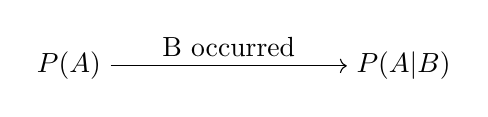
\begin{tikzpicture}
                    % Place nodes
                    \node (pA) {$P(A)$};
                    \node [right=3cm of pA] (pAcB) {$P(A|B)$};
                    % Draw edges
                    % \path[->] (pA) edge node [below,anchor=center,pos=0.25] {B occurred} (pAcB);
                    \path[->] (pA) edge node [above] {B occurred} (pAcB);
                \end{tikzpicture}
            \end{figure}

		\item Definition 1: $P(\cdot|B)=P(\cdot\cap B)$, where $\cdot$ can be any event.

		\item Problem with Definition 1: we want $P(B|B)=1$, but from Definition 1, $P(B|B)=P(B\cap B)=P(B)\le 1$.

		\item Definition 2: $P(\cdot|B)=\frac{P(\cdot\cap B)}{P(B)}$.

			\begin{itemize}
				\item $P(B|B)=1\;\checkmark$
				\item $P(A)=P(A|\Omega)=\frac{P(A\cap\Omega)}{P(\Omega)}=\frac{P(A)}{1}=P(A)\;\checkmark$
			\end{itemize}

    \end{itemize}

	\note{
		- p. 256: good motivation of conditional probability in the cards example

		- Definition 8.1

		[- interpretation of condition probability with relative frequencies]

	}
\end{frame}

\begin{frame}
    \frametitle{Definition of conditional probability}
    \label{slide:defCondProb}

    \begin{probDef}[Conditional probability]

		For any to events $A$ and $B$, with $P(B)>0$, the conditional
probability of $A$ given $B$, $P(A|B)$, is defined as 

		\begin{align*}
			P(A|B)=\frac{P(A\cap B)}{P(B)}
		\end{align*}

	\end{probDef}

\end{frame}

\begin{frame}
    \frametitle{Example 8.1: conditional probability for two dice}

	\begin{manualProbExample}{8.1}
		Someone has rolled two dice. You know that one of the dice turned up a
face value of six. What is the probability that the other die turned up a six
as  well?
	\end{manualProbExample}

	\note{

		- Example 8.1 (first ask students their intuition, as the problem is counter intuitive)

		- do NOT present example 8.2 at this point, as it requires the concept of independence

	}
\end{frame}

\begin{frame}
    \frametitle{Analytical solution of example 8.1}

    \begin{itemize}[<+->]

		\item $\Omega=\{(i_1,i_2): 1\le i_1,i_2\le6\}$. $N=36$. Equally probable outcomes.

		\item $B$=``\textit{one die turned up a face value of six}''=
$\{(6,i),(j,6),(6,6):1\le i,j\le 5\}$. $N(B)=11$. $P(B)=\frac{N(B)}{N}=\frac{11}{36}$.

		\item $A$=``\textit{the other die turned up a face value of six}''

		\item $A\cap B$=``\textit{the two dice turned up a face value of six}''=
$\{(6,6)\}$. $N(A\cap B)=1$. $P(A\cap B)=\frac{N(A\cap B)}{N}=\frac{1}{36}$.

		\item Approach 1 [definition]: $P(A|B)=\frac{P(A\cap B)}{P(B)}=\frac{1/36}{11/36}=\frac{1}{11}$.

		\item Approach 2 [$B$ as $\Omega$]: $P(A|B)=\frac{N(A\cap B)}{N(B)}=\frac{1}{11}$.

    \end{itemize}

\end{frame}

\begin{frame}[fragile]
    \frametitle{Simulated solution of example 8.1}

    Please see code \href{https://joacorapela.github.io/gcnuBridging2023/auto_examples/foundations/plot_example8_1.html#sphx-glr-auto-examples-foundations-plot-example8-1-py}{here}.

\end{frame}

\begin{frame}
    \frametitle{Exercise}

    Someone has rolled two dice. You know that the first die turned up a
face value of six. What is the probability that the second die turned up a six
as  well?

\end{frame}

\subsection{Assigning probabilities by conditioning}

\begin{frame}
    \frametitle{Assigning probabilities by conditioning}

    \scriptsize
    \begin{probRule}
        \label{rule:assignProByCond}
        For any $n\in\mathbb{N}$, $n\ge 2$, and any sequence of events $A_1,\ldots,A_n$,
            \begin{align*}
                P(A_1\cap\ldots\cap A_n) = P(A_n|A_{n-1}\cap\ldots\cap A_1)
                P(A_{n-1}|A_{n-2}\cap\ldots\cap A_1)\ldots P(A_1)
            \end{align*}
    \end{probRule}

\end{frame}

\begin{frame}
    \frametitle{Proof of rule 5}

    \tiny
    \begin{proof}
        By induction.

        \begin{description}
            \item[$P_2$:] $P(A_1\cap A_2)=P(A_2|A_1)P(A_1)$
            \item[$P_n\rightarrow P_{n+1}$:]
                \begin{align*}
                    P(A_1\cap A_2\cap\ldots\cap A_n\cap A_{n+1})=\;&P(B\cap A_{n+1})\\
                    =\;&P(A_{n+1}|B)P(B)\\
                    =\;&P(A_{n+1}|A_n\cap A_{n-1}\cap\ldots A_1)\\
                       &P(A_n\cap A_{n-1}\cap\ldots\cap A_1)\\
                    =\;&P(A_{n+1}|A_n\cap A_{n-1}\cap\ldots A_1)\\
                       &P(A_n|A_{n-1}\cap\ldots\cap A_1)\\
                       &P(A_{n-1}|A_{n-2}\cap\ldots\cap A_1)\ldots P(A_1)
                \end{align*}
        \end{description}
    \end{proof}
    Notes:
    \begin{enumerate}
        \item $P_2$ follows from the definition of conditional probability.
        \item in the first equality in $P_n\rightarrow P_{n+1}$ we defined the
            event $B=A_1\cap\ldots\cap A_n$.
        \item in the second equality in $P_n\rightarrow P_{n+1}$ we used the
            definition of conditional probability.
        \item in the third equality in $P_n\rightarrow P_{n+1}$ we replaced $B$
            by its definition.
        \item in the fourth equality in $P_n\rightarrow P_{n+1}$ we used the
            inductive hypothesis $P(A_1\cap\ldots\cap A_n) =
            P(A_n|A_{n-1}\cap\ldots\cap A_1)P(A_{n-1}|A_{n-2}\cap\ldots\cap
            A_1)\ldots P(A_1)$.
    \end{enumerate}
\end{frame}

\begin{comment}
\begin{frame}
    \frametitle{Example:}

    - redo Example 7.9 (solution following Rule 4)

\end{frame}

\begin{frame}
    \frametitle{Example:}

    - probability that it takes 10 or more cards before the first ace appears

\end{frame}
\end{comment}

\begin{frame}
    \frametitle{Example 8.3: allocating tourists to hotels}

    \footnotesize
    \begin{manualProbExample}{8.3}
        A group of 15 tourists is stranded in a city with four hotels of the
        same class. Each of the hotels has enough room available to accommodate
        the 15 tourists. The group's guide, who has a good working relationship
        with each of the four hotels, assigns the tourists to the hotels as
        follows. First, he randomly determines how many tourists will go to
        hotel A, then how many of the remaining tourists will go to hotel B, and
        next how many of the still remaining tourists will go to hotel C. All
        remaining tourists are sent to hotel D. At each stage of the assignment
        the guide draws a random number between zero and the number of tourists
        left.
        \begin{enumerate}[a]
            \item Calculate the probability of any assignment of tourists to
                hotels.
            \item Check that the probability of all possible assignments equals
                one.
            \item What is the probability that all four hotels receive guests?
            \item Is the selected rule fair to the four hotels?
        \end{enumerate}
    \end{manualProbExample}
    \normalsize

\end{frame}

\begin{frame}
    \frametitle{Analytical solution of example 8.3}

    \tiny
    Let $i$, $j$ and $k$ be the number of tourists assigned to hotels A, B an C
    respectively. Then 

    \begin{align*}
        \Omega=\{(i,j,k,15-(i+j+k)):\;&0\le i\le 15,\\
                                      &0\le j\le 15-i;\\
                                      &0\le k\le 15-(i+j)\}
    \end{align*}

    \begin{enumerate}[a]

		\item Define the events $E_j(k)$=``hotel $W$ receives $k$ tourists,''
with $W\in\{A,B,C,D\}$.

			The assignment $(i,j,k,15-(i+j+k))$ is the only member of the
            event $E_A(i)\cap E_B(j)\cap E_C(k)\cap E_D(15-(i+j+k))$. Then
            \begin{align*}
                P(\{(i,j,k,15-(i+j+k))\})&=P(E_A(i)\cap E_B(j)\cap E_C(k))\\
                                         &=P(E_C(k)|E_A(i)\cap
                                         E_B(j))\;P(E_B(j)|E_A(i))\;P(E_A(i))\\
                P(E_A(i))&=\frac{1}{16}\\
                P(E_B(j)|E_A(i))&=\frac{1}{16-i}\\
                P(E_C(k)|E_B(j)\cap E_A(i))&=\frac{1}{16-(i+j)}
            \end{align*}
            Therefore
            \begin{align*}
                P(\{(i,j,k,15-(i+j+k))\})&=\frac{1}{16-(i+j)}\frac{1}{16-i}\frac{1}{16}
            \end{align*}
		\seti
    \end{enumerate}
    \normalsize

\end{frame}

\begin{frame}
    \frametitle{Analytical solution of example 8.3}

    \tiny
    Let $i$, $j$ and $k$ be the number of tourists assigned to hotels A, B an C
    respectively. Then 

    \begin{align*}
        \Omega=\{(i,j,k,15-(i+j+k)):\;&0\le i\le 15,\\
                                      &0\le j\le 15-i;\\
                                      &0\le k\le 15-(i+j)\}
    \end{align*}

    \begin{enumerate}[a]
		\conti
        \item 
            \begin{align*}
				P(\Omega)&=\sum_{\omega\in\Omega}P(\omega)=\sum_{i=0}^{15}\sum_{j=0}^{15-i}\sum_{k=0}^{15-(i+j)}P(\{(i,j,k,15-(i+j+k))\})\\
                         &=\sum_{i=0}^{15}\sum_{j=0}^{15-i}\sum_{k=0}^{15-(i+j)}\frac{1}{16-(i+j)}\frac{1}{16-i}\frac{1}{16}\\
                         &=\frac{1}{16}\sum_{i=0}^{15}\frac{1}{16-i}\sum_{j=0}^{15-i}\frac{1}{16-(i+j)}\sum_{k=0}^{15-(i+j)}1\\
                         &=\frac{1}{16}\sum_{i=0}^{15}\frac{1}{16-i}\sum_{j=0}^{15-i}\frac{1}{16-(i+j)}(16-(i+j))\\
                         &=\frac{1}{16}\sum_{i=0}^{15}\frac{1}{16-i}\sum_{j=0}^{15-i}1=\frac{1}{16}\sum_{i=0}^{15}\frac{1}{16-i}(16-i)=\frac{1}{16}\sum_{i=0}^{15}1=\frac{1}{16}16=1
            \end{align*}
		\seti
    \end{enumerate}
    \normalsize

\end{frame}

\begin{frame}
    \frametitle{Analytical solution of example 8.3}

    \tiny
    \begin{enumerate}[a]
		\conti
        \item 
			Define the event $E$=``all hotels receive guests.'' Then
    		\begin{align*}
        		E=\{(i,j,k,15-(i+j+k)):\;&1\le i\le 12,\\
                                      	 &1\le j\le 13-i;\\
                                      	 &1\le k\le 14-(i+j)\}
            \end{align*}
    		\begin{align*}
				P(E)&=\sum_{i=1}^{12}\sum_{j=1}^{13-i}\sum_{k=1}^{14-(i+j)}P(\{(i,j,k,15-(i+j+k))\})\\
                    &=\sum_{i=1}^{12}\sum_{j=1}^{13-i}\sum_{k=1}^{14-(i+j)}\frac{1}{16-(i+j)}\frac{1}{16-i}\frac{1}{16}\\
                    &=0.2856
            \end{align*}
        \item
    		\begin{align*}
                P(\{(15,0,0,0)\})&=\frac{1}{16}\\
                P(\{(0,15,0,0)\})&=\frac{1}{16^2}
            \end{align*}
            Thus, the selected rule is unfair to the four hotels.
    \end{enumerate}
    \normalsize

\end{frame}

\begin{frame}[fragile]
    \frametitle{Simulated solution of example 8.3c}

    Please see code \href{https://joacorapela.github.io/gcnuBridging2023/auto_examples/foundations/plot_example8_3.html#sphx-glr-auto-examples-foundations-plot-example8-3-py}{here}.

\end{frame}

\subsection{Independent events}

\begin{frame}
    \frametitle{Independent events}
    \scriptsize

    If event $A$ is independent from event $B$, then knowing that $B$ has
    occurred does not change the probability that event $A$ occurs.

    \begin{probDef}
        Two events $A$ and $B$ are independent if
        \begin{align*}
            P(A|B)=P(A)
        \end{align*}
    \end{probDef}
    
    \onslide<2->{
    \begin{claim*}
        If events $A$ and $B$ are independent if and only if
        \begin{align*}
            P(A\cap B)=P(A)P(B)
        \end{align*}
    \end{claim*}
    }

    \onslide<3->{
    \begin{proof}
        $\rightarrow$: $P(A\cap B)=P(A|B)P(B)=P(A)P(B)$

        \vspace{0.1in}
        $\leftarrow$: $P(A|B)=\frac{P(A\cap B)}{P(B)}=\frac{P(A)P(B)}{P(B)}=P(A)$
    \end{proof}
    }

    \normalsize

    \note{

        - motivation of independence definition with conditional probabilities

        - Definition 8.2

    }

\end{frame}

\begin{frame}
    \frametitle{Example 8.5: independent dice events?}

    \begin{manualProbExample}{8.5}
        Two fair dice are thrown. Let $A$ be the event that the number shown in
        die one is even, and $B$ the event that the sum of the two dice
        is odd. Are $A$ and $B$ independent?
    \end{manualProbExample}

\end{frame}

\begin{frame}
    \frametitle{Analytical solution of example 8.5}

    \scriptsize
    The sample space is

    \begin{alignat*}{3}
        \Omega&=\{&&(d_1, s): d_1\text{ number shown in die one, }s\text{ sum of the two dice}\}\\
              &=\{&&(1,2),(1,3),\ldots,(1,7),\\
              &   &&(2,3),(2,4),\ldots,(2,8),\\
              &   &&\ldots,\\
              &   &&(6,7),(6,8),\ldots,(6,12)\}\\
        N(\Omega)&=&&36,N(A)=N(B)=18,N(A\cap B)=9\\
        P(B)&=     &&\frac{N(B)}{N(\Omega)}=\frac{18}{36}=\frac{1}{2}\\
        P(B|A)&=   &&\frac{N(A\cap B)}{N(A)}=\frac{9}{18}=\frac{1}{2}
    \end{alignat*}

    Since $P(B)=P(B|A)$, events $A$ and $B$ are independent.
    \normalsize
\end{frame}

\begin{frame}
    \frametitle{Exercise: independence-related proofs}

    Prove the following claims:

    \begin{claim*}[disjoint events are generally not independent]

        Let $A$ and $B$ be two events and $P$ a probability measure such that
        $P(A)\ne 0$ and $P(B)\ne 0$. Then, it is always true that the fact that
        $A$ and $B$ are disjoint implies that $A$ and $B$ are not independent.

    \end{claim*}

    \begin{claim*}[symmetry of independence]
        $P(A|B)=P(A)$ if and only if $P(B|A)=P(B)$.
    \end{claim*}
\end{frame}

\begin{comment}
\begin{frame}
    \frametitle{Example}

- Example 8.6 (uses birthday problem, example 7.10)

\end{frame}
\end{comment}

\subsection{Conditionally independent events}

\begin{frame}
    \frametitle{Conditionally independent events}
    \label{slide:conditionallyIndependentEvents}

    \begin{probDef}
        Events $A$ and $B$ are conditionally independent given event $C$ if and
        only if $P(A|B\cap C)=P(A|C)$.
    \end{probDef}

\end{frame}

\begin{frame}
    \frametitle{Example on conditional independence}

    \scriptsize
    \begin{manualProbExample}{tossing a possibly unfair coin}

        Suppose both Martin and Norman toss the same coin. Let $A$ be the event
        ``Norman's toss resulted in heads'', and $B$ the event ``Martin's toss
        resulted in heads.'' Assume also that there is a possibility that the
        coin in biased towards heads but we do not know this for certain.  In
        this case events $A$ and $B$ are not independent. For example, observing
        that B occurred causes us to increase our belief that A occurred (i.e.,
        $P(A|B)>P(A)$).

        In the above, events $A$ and $B$ are dependent on event $C$, ``the coin
        is biased towards heads.'' Although events $A$ and $B$ are not
        independent, it turns out that they are conditionally independent given
        event $C$, i.e., once we know for certain that event C occurred then
        any evidence about $B$ cannot change our belief about $A$ (i.e.,
        $P(A|C) = P(A|B\cap C)$).

    \end{manualProbExample}
    \normalsize

\end{frame}

\begin{frame}
    \frametitle{Example on conditional independence}

    \scriptsize
    \begin{manualProbExample}{tossing a possibly unfair coin}

        Let's assign probabilities to the events above and verify the claims
        that (a) events $A$ and $B$ are dependent (i.e., $P(A|B)>P(A)$) and
        that (b) events $A$ and $B$ are conditionally independent given event
        $C$ (i.e., $P(A|B\cap C)=P(A|B)$).

        \begin{enumerate}[a]

            \item list the elements of the sample space $\Omega$, and of events $A$, $B$ and $C$.

            \item assign probabilities to events containing only one element of
                $\Omega$, so that 

                \begin{itemize}
                    \scriptsize

                    \item events $A$ and $B$  and events $A$ and $B^c$ are
                        conditionally independent given that the coin is biased
                        or given that the coin is unbiased,

                    \item the probability of heads given that the coin is
                        biased is 0.7

                    \item the coin is equally likely biased or unbiaed.

                \end{itemize}

            \item with the previous assigned probabilities, check that events
                $A$ and $B$ are not independent but that they are conditionally
                independent given $C$.

        \end{enumerate}

    \end{manualProbExample}
    \normalsize

\end{frame}

\begin{frame}
    \frametitle{Analytical solution of example on conditional independence}

    \scriptsize
    \begin{enumerate}[a]

        \item
            \begin{align*}
                \Omega&=\{\text{HHU,HTU,THU,TTU,HHB,HTB,THB,TTB}\}\\
                A&=\{\text{HHU,HTU,HHB,HHB}\}\\
                B&=\{\text{HHU,THU,HHB,HHB}\}\\
                C&=\{\text{HHB,HTB,THB,TTB}\}
            \end{align*}

            In the above, for example, HTB means that Norman tossed a heads,
            Martin tossed a tail and the coin was biased towards heads.

            \seti
    \end{enumerate}
\end{frame}

\begin{frame}
    \frametitle{Analytical solution of example on conditional independence}

    \scriptsize
    \begin{enumerate}[a]
        \conti
        \item

            Given the example setup we know that

            \begin{align*}
                P(A|C^c)&=P(B|C^c)=\frac{1}{2}\\
                P(A|C)&=P(B|C)=\frac{1}{7}\\
                P(C)&=P(C^c)=\frac{1}{2}\\
                P(A|B,C^c)&=P(A|B^c,C^c)=P(A|C^c)\\
                P(A|B,C)&=P(A|B^c,C)=P(A|C)
            \end{align*}
            
    \end{enumerate}
    \normalsize

\end{frame}

\begin{frame}
    \frametitle{Analytical solution of example on conditional independence}

    \scriptsize
    \begin{enumerate}[a]

        \conti
        \item
            Next we will assign probabilities uing
            Rule~\ref{rule:assignProByCond},

            \begin{align*}
                P(\{HHU\})&=P(A\cap B\cap C^c)=P(A|B\cap C^c)P(B|C^c)P(C^c)\\
                          &=P(A|C^c)P(B|C^c)P(C^c)=\frac{1}{2}\frac{1}{2}\frac{1}{2}=\frac{1}{8}
                % P(\{HTU\})=P(A\cap B^c\cap C^c)=P(A|B^c\cap C^c)P(B^c|C^c)P(C^c)=P(A|C^c)P(B^c|C^c)P(C^c)=\frac{1}{2}\frac{1}{2}\frac{1}{2}=\frac{1}{8}
            \end{align*}

            The second equality above uses Rule~\ref{rule:assignProByCond}, and
            the third equality uses the fact that $A$ is conditionally
            independent from $B$ given $C^c$.

            In the same way we can see that
            $P(\{HTU\})=P(\{THU\})=P(\{TTU\})=\frac{1}{8}$.

    \end{enumerate}
    \normalsize

\end{frame}

\begin{frame}
    \frametitle{Analytical solution of example on conditional independence}

    \scriptsize
    \begin{enumerate}[a]

        \conti
        \item
            For a biased coin we have

            \begin{align*}
                P(\{HHB\})&=P(A\cap B\cap C)=P(A|B\cap C)P(B|C)P(C)\\
                          &=P(A|C)P(B|C)P(C)=\frac{7}{10}\frac{7}{10}\frac{1}{2}=\frac{49}{200}\\
                P(\{HTB\})&=P(A\cap B^c\cap C)=P(A|B^c\cap C)P(B^c|C)P(C)\\
                          &=P(A|C)P(B^c|C)P(C)=P(A|C)(1-P(B|C))P(C)\\
                          &=\frac{7}{10}\frac{3}{10}\frac{1}{2}=\frac{21}{200}\\
                P(\{THB\})&=P(A^c\cap B\cap C)=P(A^c|B\cap C)P(B|C)P(C)\\
                          &=P(A^c|C)P(B|C)P(C)=(1-P(A|C))P(B|C)P(C)\\
                          &=\frac{3}{10}\frac{7}{10}\frac{1}{2}=\frac{21}{200}\\
                P(\{TTB\})&=P(A^c\cap B^c\cap C)=P(A^c|B^c\cap C)P(B^c|C)P(C)\\
                          &=P(A^c|C)P(B^c|C)P(C)=(1-P(A|C))(1-P(B|C))P(C)\\
                          &=\frac{3}{10}\frac{3}{10}\frac{1}{2}=\frac{9}{200}
            \end{align*}
    \end{enumerate}
    \normalsize

\end{frame}

\begin{frame}
    \frametitle{Analytical solution of example on conditional independence}

    \tiny
    \begin{enumerate}[a]

        \conti
        \item
            Thus, the probabilities of single-outcome events are:

            \setlength{\tabcolsep}{2pt}
            \begin{tabular}{|c|c|c|c|c|c|c|c|}
                \hline
                $\{HHU\}$ & $\{HTU\}$ & $\{THU\}$ & $\{TTU\}$ & $\{HHB\}$ & $\{HTB\}$ & $\{THB\}$ & $\{TTB\}$\\
                \hline\hline
                $\frac{1}{8}$ & $\frac{1}{8}$ & $\frac{1}{8}$ & $\frac{1}{8}$ & $\frac{49}{200}$ & $\frac{21}{200}$ & $\frac{21}{200}$ & $\frac{9}{200}$\\
                \hline
            \end{tabular}

        \item
            \begin{align*}
                P(A|B)&=\frac{P(A\cap B)}{P(B)}=
                \frac{P((A\cap B)\cap (C\cup C^c))}{P(B\cap ((A\cap C)\cup (A\cap C^c)\cup (A^c\cap C)\cup (A^c\cap C^c))}\\
                &=\frac{P((A\cap B\cap C)\cup (A\cap B\cap C^c))}{P((B\cap A\cap C)\cup (B\cap A\cap C^c)\cup (B\cap A^c\cap C)\cup (B\cap A^c\cap C^c))}\\
                &=\frac{P(A\cap B\cap C)+P(A\cap B\cap C^c)}{P(B\cap A\cap C)+P(B\cap A\cap C^c)+P(B\cap A^c\cap C)+P(B\cap A^c\cap C^c))}\\
                &=\frac{P(\{HHB\})+P(\{HHU\})}{P(\{HHB\})+P(\{HHU\})+P(\{THB\})+P(\{THU\})}\\
                &=\frac{\frac{49}{200}+\frac{1}{8}}{\frac{49}{200}+\frac{1}{8}+\frac{21}{200}+\frac{1}{8}}=\frac{\frac{74}{200}}{\frac{120}{200}}=\frac{74}{120}=0.62\\
                P(A)&=P(B)=\frac{120}{200}=0.6<0.62=P(A|B)\quad\text{Therefore, A and B are not independent.}
            \end{align*}
            \seti
    \end{enumerate}
    \normalsize

\end{frame}

\begin{frame}
    \frametitle{Analytical solution of example on conditional independence}

    \tiny
    \begin{enumerate}[a]

        \keepi
        \item
            \begin{align*}
                P(A|B\cap C)&=\frac{P(A\cap B\cap C)}{P(B\cap C)}=
                \frac{P(A\cap B\cap C)}{P((B\cap C)\cap (A\cup A^c))}=
                \frac{P(A\cap B\cap C)}{P((A\cap B\cap C)\cup (A^c\cap B\cap
                C))}\\
                &=\frac{P(A\cap B\cap C)}{P(A\cap B\cap C)+P(A^c\cap B\cap C)}=
                \frac{P(\{HHB\})}{P(\{HHB\}+P(\{THB\})}=\frac{\frac{49}{200}}{\frac{49}{200}+\frac{21}{200}}=\frac{7}{10}\\
                P(A|C)&=\frac{P(A\cap C)}{P(C)}=\frac{P((A\cap C)\cap (B\cup
                B^c))}{P(C\cap ((A\cap B)\cup (A\cap B^c)\cup (A^c\cap B)\cup
                (A^c\cap B^c))}\\
                &=\frac{P((A\cap B\cap C)\cup (A\cup B^c\cap C))}{P((A\cap
                B\cap C)\cup (A\cap B^c\cap C)\cup (A^c\cap B\cap C)\cup
                (A^c\cap B^c\cap C))}\\
                &=\frac{P(A\cap B\cap C)+P(A\cup B^c\cap C)}{P(A\cap
                B\cap C)+P(A\cap B^c\cap C)+P(A^c\cap B\cap C)+P(A^c\cap B^c\cap C)}\\
                &=\frac{P(\{HHB\})+P(\{HTB\})}{P(\{HHB\})+P(\{HTB\})+P(\{THB\})+P(\{TTB\})}\\
                &=\frac{\frac{49}{200}+\frac{21}{200}}{\frac{49}{200}+\frac{21}{200}+\frac{21}{200}+\frac{9}{200}}\\
                &=\frac{\frac{70}{200}}{\frac{100}{200}}=\frac{7}{10}=P(A|B\cap
                C)\quad\text{Therefore, A and B are conditionally independent given C.}
            \end{align*}
    \end{enumerate}
    \normalsize

\end{frame}

\subsection{Law of conditional probability}

\begin{frame}
    \frametitle{Example p86: dice followed by coin tosses}

    \begin{manualProbExample}{page 266}
        A fair die is rolled to yield a number between one and six, and then a
        coin is tossed that many times. What is the probability that heads will
        not appear?
    \end{manualProbExample}

\end{frame}

\begin{frame}
    \frametitle{Analytical solution of example p86}
    \tiny
    \begin{align*}
        P(\text{no\_heads})&=P(\text{no\_heads}\cap\Omega)\\
                           &=P(\text{no\_heads}\cap\left(\text{die\_equals\_1}\cup\text{die\_equals\_2}\cup\dots\cup\text{die\_equals\_6}\right))\\
                           &=P((\text{no\_heads}\cap\text{die\_equals\_1})\cup (\text{no\_heads}\cap\text{die\_equals\_2})\cup\ldots\cup (\text{no\_heads}\cap\text{die\_equals\_6})))\\
                           &=\sum_{i=1}^6P(\text{no\_heads}\cap\text{die\_equals\_i})=\sum_{i=1}^6P(\text{no\_heads}|\text{die\_equals\_i})P(\text{die\_equals\_i})\\
                           &=P(T)P(\text{die\_equals\_1})+
                           P(TT)P(\text{die\_equals\_2})+\ldots +
                           P(TTTTTT)P(\text{die\_equals\_6})\\
                           &=\frac{1}{2}\frac{1}{6}+\left(\frac{1}{2}\right)^2\frac{1}{6}+\ldots+\left(\frac{1}{2}\right)^6\frac{1}{6}=0.1640625
    \end{align*}
    \normalsize

\end{frame}

\begin{comment}
\begin{frame}
    \frametitle{Analytical solution of example p86}
    \tiny
    \begin{align*}
        \Omega=\{&(d=1,c=H),(d=1,c=T),\\
                 &(d=2,c=HH),(d=2,c=TH),(d=2,c=HT),(d=2,c=TT),\\
                 &\ldots,\\
                 &(d=6,c=HHHHHH),\ldots,(d=6,c=TTTTTT)\}
    \end{align*}

    Let's define a few events

    \begin{align*}
        \text{no\_heads}=\{((d=1,c=H),(d=2,c=TT),(d=3,c=TTT),\ldots\}
    \end{align*}
    \normalsize

\end{frame}
\end{comment}

\begin{frame}[fragile]
    \frametitle{Simulated solution of example p86}

    Please see code
    \href{https://joacorapela.github.io/gcnuBridging2023/auto_examples/foundations/plot_examplep86.html#sphx-glr-auto-examples-foundations-plot-examplep86-py}{here}.

\end{frame}

\begin{frame}
    \frametitle{Law of conditional probability}

    \begin{probRule}
        \textbf{Law of conditional probability} Let $A$ be an event that
            can only occur if one of the mutually exclusive events
            $B_1,\ldots,B_n$ occurs. Then

            \begin{align*}
                P(A) = P(A|B_1) P(B_1) + \ldots + P(A|B_n) P(B_n)  
            \end{align*}
    \end{probRule}

\end{frame}

\begin{frame}
    \frametitle{Exercise: proof of law of conditional probability}

    Prove the law of conditional probability. Hint: use induction as in the
    proof of rule 5.

\end{frame}

\begin{frame}
    \frametitle{Exercise: tour de France}

    \begin{manualProbExample}{8.6}
        The upcoming Tour the France bicycle tournament will take place from
        July 1 through July 23. One hundred and eighty cyclists will
        participate in event. What is the probability that two or more
        participating cyclists will have birthdays on the same day during the
        tournament?
    \end{manualProbExample}

\end{frame}

\section{Statistical inference}

\begin{comment}
\subsection{Bayes's rule in odds form}

\begin{frame}
    \frametitle{Bayes rule in odds form}

- true/false hypothesis

    \begin{description}

        \item{Rule 6} The posterior probability $P(H|E)$ satisfies

            \begin{align*}
                \frac{P(H|E)}{P(\bar{H}|E)} = \frac{P(H)}{P(\bar{H})}\frac{P(E|H)}{P(E|\bar{H})}
            \end{align*}

    \end{description}

- interpretation of rule 6

    - avoid need of P(E)

    - prior odds + likelihood ratio or Bayes factor

    - prior odds update with new evidence

    - sequential update (mention Bayesian linear regression)

\end{frame}

\begin{frame}
    \frametitle{Example}

- example 8.8

\end{frame}

\begin{frame}
    \frametitle{Example}

- example 8.11

    - add to the problem statement:

        - in 1992, 4936 women were murdered in the US, of which roughly 1430 were murdered by their (ex)husbands or boyfriends

        - 5\% of the married women in the US have at some point been physically abused by their husbands.

        - assume that a woman who has been murdered by some other than her husband had the same same chance of being abused by her husband as a randomly selected woman

        - Alan Dershowitz admitted that a substantial percentage of the husbands who murder their wives, previous to the murder, also physically abuse their wives. Given this statement, we assume that the probability that a husband physically abused his wife, given that he killed her, is 50 percent.

\end{frame}

\end{comment}

\subsection{Bayesian inference -- discrete case}

\begin{frame}
    \frametitle{Bayesian inference}

    \begin{itemize}

        \item In Bayesian statistics parameters of a model, $\theta$ are considered random quantities. They are assigned a (subjective) probability $P(\theta)$.

        \item The probability of parameters is subject to change as new data arrives, $P(\theta|D)$.

            \begin{figure}
                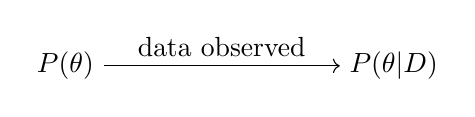
\begin{tikzpicture}
                    % Place nodes
                    \node (pTheta) {$P(\theta)$};
                    \node [right=3cm of pTheta] (pThetaGivenD) {$P(\theta|D)$};
                    % Draw edges
                    \path[->] (pTheta) edge node [above] {data observed} (pThetaGivenD);
                \end{tikzpicture}
            \end{figure}

        \item How to calculate the posterior probability $P(\theta|D)$?

            \begin{align*}
                P(\theta|D)&=\frac{P(\theta\cap D)}{P(D)}\\
                P(\theta\cap D)&=P(D|\theta)P(\theta)\\
%                 \text{Thus}&\\
                P(\theta|D)&=\frac{P(D|\theta)P(\theta)}{P(D)}\propto P(D|\theta)P(\theta)\\
            \end{align*}

    \end{itemize}

\end{frame}

\begin{frame}
    \frametitle{Bayesian inference}

    \scriptsize
    \begin{itemize}

        \item Sequential update

        \begin{align*}
            P(\theta|D_1\cap D_2)&=\frac{P(\theta\cap D_1\cap D_2)}{P(D_1\cap D_2)}\\
                                 &=\frac{P(D_2|D_1\cap\theta)P(D_1\cap\theta)}{P(D_1\cap D_2)}\\
                                 &=\frac{P(D_2|\theta)P(D_1|\theta)P(\theta)}{P(D_1\cap D_2)}\\
                                 &=K\;P(D_2|\theta)P(\theta|D_1)\propto P(D_2|\theta)P(\theta|D_1)
        \end{align*}

        Notes:

        \begin{enumerate}

            \item the first and second equalities use the
                \hyperlink{slide:defCondProb}{definition of conditional
                probability}.

            \item the third equality assumes that the datasets $D_1$ and $D_2$
                are
                \hyperlink{slide:conditionallyIndependentEvents}{conditionally
                independent} given $\theta$.

            \item the last equality groups all factors that don't depend on
                $\theta$ in the proportionality constant $K$.

        \end{enumerate}

    \end{itemize}
    \normalsize

\end{frame}

\begin{frame}
    \frametitle{Exercise: sequential posterior probability for arbitrary number of observations}

    For any $n\in\mathbb{N}$, prove that

    \begin{align*}
        P(\theta|D_1\cap\ldots\cap D_{n+1})=P(D_{n+1}|\theta)P(\theta|D_1\cap D_2\cap\ldots\cap D_n)
    \end{align*}

\end{frame}

\begin{frame}
    \frametitle{Example 8.13: disease treatment effect}

	\small
    \begin{manualProbExample}{8.13}

        A new treatment is tried out for a disease. A standard treatment has a
        success probability of 35\%. The discrete uniform distribution on 0.00,
        0.01, \ldots, 0.99, 1.00 is taken as prior for the success probability
        of the new treatment. The experiment design is to make exactly ten
        observations by treating ten patients. The experimental study yield
        seven successes and three failures~\citep{berry06}.

		\begin{enumerate}[a]

			\item Plot the prior of the success probability of the new treatment.
			\item Plot the likelihood of the success probability of the new treatment.
			\item Plot the posterior of the success probability of the new treatment.
			\item What is the posterior probability that the new treatment is
			more effective than the standard one?

		\end{enumerate}

    \end{manualProbExample}
	\normalsize

\end{frame}

\begin{frame}
    \frametitle{Analytical solution of example 8.13}

    \scriptsize
	\begin{enumerate}[a]

		\item prior:

			\begin{align*}
				p(\theta) = \frac{1}{101},\quad\text{for}\;\theta=0.00,0.01,\ldots,0.99,1.00
			\end{align*}
            \seti
	\end{enumerate}

\end{frame}

\begin{frame}
    \frametitle{Analytical solution of example 8.13}

    \tiny
	\begin{enumerate}[a]
        \conti
		\item likelihood:

			\begin{align*}
				\Omega&=\{(r_1,\ldots,r_{10}):r_i\in\{S,F\}\}
			\end{align*}

			Define the events \textit{k\_successes}=``experiments where k out of the 10 observations were successes'', with $k\in\{0,1,\ldots,10\}$.

            \begin{alignat*}{2}
                \text{0\_successes}&=\{&&(F,F,F,F,F,F,F,F,F,F)\}\\
                \text{1\_successes}&=\{&&(S,F,F,F,F,F,F,F,F,F),(F,S,F,F,F,F,F,F,F,F),\ldots,\\
                                   &   &&(F,F,F,F,F,F,F,F,F,S)\}\\
                \text{2\_successes}&=\{&&(S,S,F,F,F,F,F,F,F,F),(S,F,S,F,F,F,F,F,F,F),\ldots,\\
                                   &   &&(F,F,F,F,F,F,F,F,S,S)\}
            \end{alignat*}

            Calculate the events probabilities

			\begin{alignat*}{2}
				P(0\_successes|\theta)=&P(\{&&(F,F,F,F,F,F,F,F,F,F)\})=(1-\theta)^{10}\\
				P(1\_successes|\theta)=&P(\{&&(S,F,F,F,F,F,F,F,F,F),(F,S,F,F,F,F,F,F,F,F),\ldots,\\
                                      &    &&(F,F,F,F,F,F,F,F,F,S)\}\})\\
                                     =&P(\{&&(S,F,F,F,F,F,F,F,F,F)\})+P(\{(F,S,F,F,F,F,F,F,F,F)\})+\ldots+\\
                                      &P(\{&&(F,F,F,F,F,F,F,F,F,S)\})=10P(\{(S,F,F,F,F,F,F,F,F,F)\})\\
                                     =&10&&\theta(1-\theta)^9
			\end{alignat*}

	\end{enumerate}
\end{frame}

\begin{frame}
    \frametitle{Analytical solution of example 8.13}

    \tiny
	\begin{enumerate}[a]
        \conti
		\item likelihood:
			\begin{alignat*}{2}
				P(2\_successes|\theta)=&P(\{&&(S,S,F,F,F,F,F,F,F,F),(S,F,S,F,F,F,F,F,F,F),\ldots,\\
                                      &    &&(F,F,F,F,F,F,F,F,S,S)\}\})\\
                                     =&P(\{&&(S,S,F,F,F,F,F,F,F,F)\})+\\
                                      &P(\{&&(S,F,S,F,F,F,F,F,F,F)\})+\ldots+\\
                                      &P(\{&&(F,F,F,F,F,F,F,F,S,S)\})\\
                                     =&\binom{10}{2}&&P(\{(S,F,F,F,F,F,F,F,F,F)\})\\
                                     =&\binom{10}{2}&&\theta^2(1-\theta)^8\\
			    P(k\_successes|\theta)=&\binom{10}{k}&&\theta^k(1-\theta)^{10-k},\quad k\in\{0,1,\ldots,10\}
			\end{alignat*}
            \seti

	\end{enumerate}
\end{frame}

\begin{frame}
    \frametitle{Analytical solution of example 8.13}

    \tiny
	\begin{enumerate}[a]
        \conti
		\item posterior:

			\begin{align*}
				P(\theta|\text{7\_successes})&=K_1P(\text{7\_successes}|\theta)P(\theta)=K_1\binom{10}{7}\theta^7(1-\theta)^3\frac{1}{101}=K_2\theta^7(1-\theta)^3\\
                1&=\sum_{k=0}^{100}P(\theta_k|\text{7\_successes})=K_2\sum_{k=0}^{100}\theta_k^7(1-\theta_k)^3;\quad\theta_k=\frac{k}{100}\\
                K_2&=\frac{1}{\sum_{k=0}^{100}\theta_k^7(1-\theta_k)^3}\\
                P(\theta|\text{7\_successes})&=\frac{\theta^7(1-\theta)^3}{\sum_{k=0}^{100}\theta_k^7(1-\theta_k)^3}
			\end{align*}

		\item 

            \begin{align*}
                P(\text{new treatment more effective than standard one})=\sum_{k=36}^{100}P(\theta_k|\text{7\_successes})
            \end{align*}

	\end{enumerate}
\end{frame}

\begin{frame}
    \frametitle{Exercise: sequential posterior probability}

    Continuing example 8.13, calculate the posterior probability of the new
    treatment after a second observation with six successes and a first
    observation with seven successes.

\end{frame}

\begin{frame}
    \frametitle{July 19: online Bayesian linear regression}

    \begin{center}
        \href{figures/onlineBayesianLinearRegression_nSamples20.html}{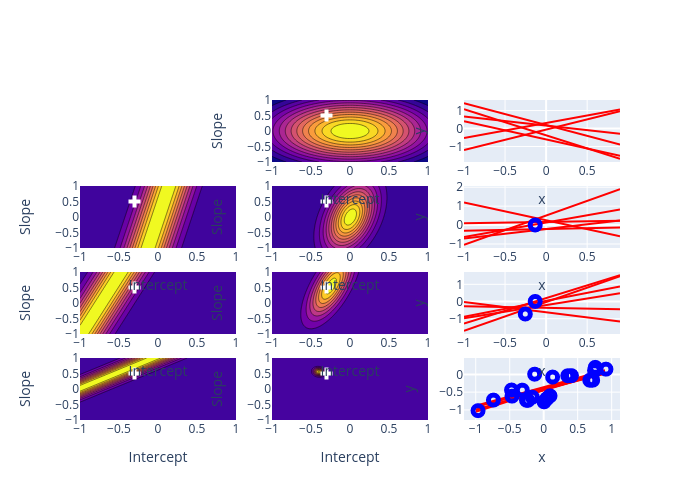
\includegraphics[width=4in]{figures/onlineBayesianLinearRegression_nSamples20.png}}
    \end{center}

\end{frame}

\begin{frame}
    \frametitle{References}

    \tiny{
        \bibliographystyle{apalike}
        \bibliography{probability}
    }
\end{frame}

\begin{comment}
\end{comment}

\end{document}

